
\begin{frame}[fragile]{Le modèle Entité / Association}

Cette session présente les notions de base du modèle entité / association

\vfill

\begin{redbullet}
  \item Présentation commentée du schéma de la base Films
  \item Entités
  \item Association un-à-plusieurs
  \item Association plusieurs-plusieurs
  \item Réification d'une association
\end{redbullet}

\vfill
\begin{blocgauche}
\alert{Ces diapositives correspondent au support en ligne disponible sur
le site \url{http://sql.bdpedia.fr/}}
\end{blocgauche}

\end{frame}


\begin{frame}{Schéma E/A commenté: la base des films}

\vspace*{0.3cm}


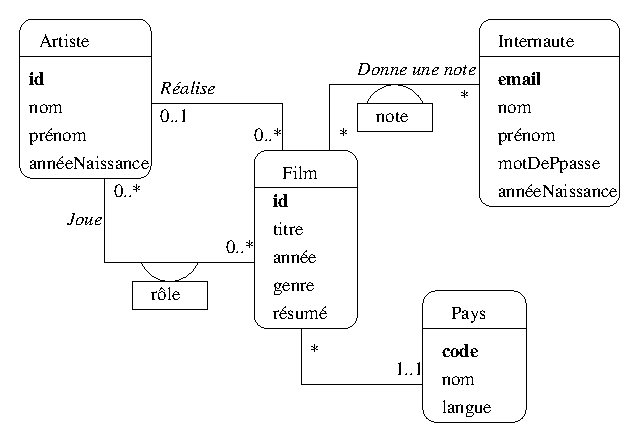
\includegraphics[width=10cm]{../../figures/films}
\end{frame}


\begin{frame}{Les types d'entité}

\begin{center}
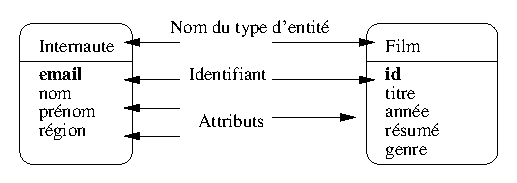
\includegraphics[width=8cm]{../../figures/entite}
\end{center}
\vfill

\begin{blocgauche}
\begin{redbullet}
  \item Tous les attributs sont \alert{atomiques}
  \item Choix de la clé: un attribut non-descriptif \texttt{id} est à peu près \alert{toujours}
      le meilleur choix.
    \item Tous les attributs doivent dépendre (fonctionnellement) directement de la clé.
\end{redbullet}
\end{blocgauche}

\end{frame}


\begin{frame}{Association binaires}

Etudions l'association "un artiste réalise un film", avec quelques exemples.

\vfill

\begin{center}
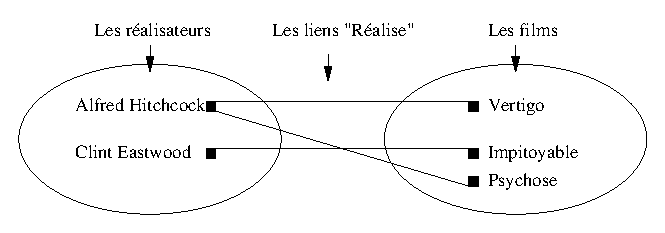
\includegraphics[width=8cm]{../../figures/graphe-ea}
\end{center}
\vfill

Décisions à prendre:

\begin{redbullet}
  \item certains réalisateurs mettent en scène plusieurs films ;
    \item inversement, un film est mis en scène par au plus un réalisateur.
\end{redbullet}

\vfill

Ces choix sont \alert{essentiels} (et difficiles à changer après coup).
\end{frame}


\begin{frame}{Cardinalités}
On représente les choix de conception sur les associations par
des \alert{cardinalités}.

\vfill
La cardinalité de l'association pour un type d'entité $E$
    est une paire $[min, max]$  :


\begin{redbullet}
  \item $max$ (cardinalité maximale)
      désigne le nombre \alert{maximal} de fois où une 
      une entité $e$ de $E$  peut intervenir dans l'association (1 ou *, nombre indéterminé).
      
    \item $min$  (cardinalité minimale)
       désigne  le nombre \alert{minimal} de fois où une 
       une entité $e$ de $E$ peut intervenir dans l'association
       (0 ou 1)
\end{redbullet}

\end{frame}


\begin{frame}{Association un-à-plusieurs (ou plusieurs-à-un)}

Représentation de l'association "un artiste réalise un film".

\vfill

\begin{center}
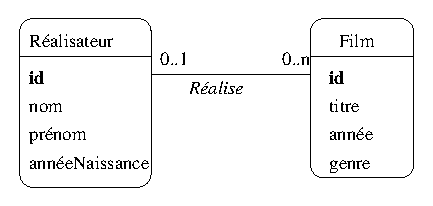
\includegraphics[width=7cm]{../../figures/assoc}
\end{center}

\vfill

\begin{blocgauche}
On interdit donc qu'un film ait deux réalisateurs.

\bigskip

On autorise qu'un film n'ait pas de réalisateur (ou qu'on ne le connaisse pas)

\end{blocgauche}
\end{frame}


\begin{frame}{Autre exemple}

Etudions l'association "un artiste joue un rôle dans un film", avec quelques exemples.

\vfill

\begin{center}
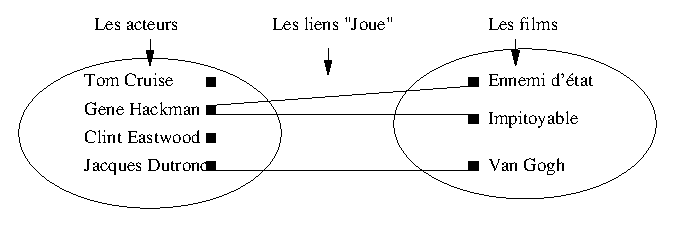
\includegraphics[width=8cm]{../../figures/graphe-ea2}
\end{center}
\vfill

Décisions à prendre:

\begin{redbullet}
  \item certains artistes jouent  dans plusieurs films ;
    \item un film peut employer plusieurs acteurs 
\end{redbullet}

\end{frame}


\begin{frame}{Association plusieurs-à-plusieurs}

Ajout  de l'association "un artiste joue dans un film".

\vfill

\begin{center}
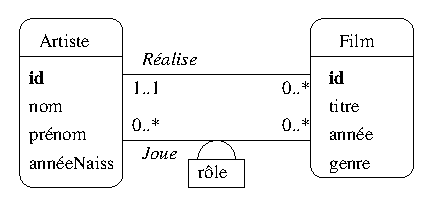
\includegraphics[width=7cm]{../../figures/assoc2}
\end{center}

\vfill

\begin{blocgauche}
Une association est identifiée par les deux entités qu'elle lie, et donc par
la paire des identifiants (idFilm, idArtiste).

\medskip

Donc, un même acteur joue \alert{au plus} un rôle dans un même film.

\end{blocgauche}


\end{frame}

%%%%%%%%
\begin{frame}{Autre exemple}

Ajout  de l'association "un internaute note des films".

\vfill

\begin{center}
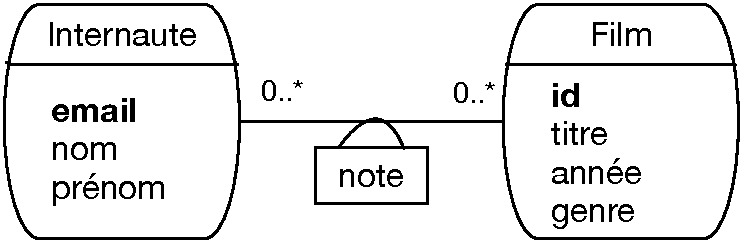
\includegraphics[width=7.5cm]{../figures-sql/assoc-internaute}
\end{center}

\vfill
\begin{blocgauche}
Un même internaute note un même film une seule fois
\end{blocgauche}

\end{frame}


%%%%%%%%
\begin{frame}{Réification des associations plusieurs-à-plusieurs}

On peut \alert{remplacer} une association plusieurs-à-plusieurs par une \alert{entité}
et des associations un-à-plusieurs.
\vfill

\begin{center}
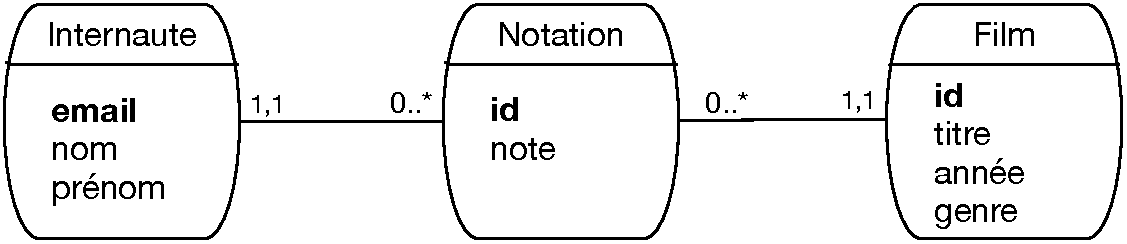
\includegraphics[width=10cm]{../figures-sql/assoc-reifiee}
\end{center}

\vfill
\begin{blocgauche}
Souvent un bon choix: il est plus facile d'exprimer des contraintes sur une entité
que sur une association.
\end{blocgauche}
\end{frame}
%%%%%%ù

\begin{frame}{À retenir}

Le modèle entité association
\vfill
\begin{redbullet}
  \item Entité: objets autonomes, identifiables, persistants.
 \item Associations: liens entre entités, caractérisées par des \alert{cardinalités}
 \item On peut toujours se ramener à des associations un-à-plusieurs.
\end{redbullet}

\vfill

\begin{blocgauche}
\alert{Ne représente pas la réalité fidèlement ou complètement} mais en fonction d'un \alert{besoin}
\end{blocgauche}
\end{frame}

